\documentclass{beamer}
\usepackage[french]{babel}
\usepackage[utf8]{inputenc}
\usepackage{amsmath, amssymb}
\usepackage{graphicx}
\usepackage{booktabs}
\usepackage{xcolor}
\usepackage{fontawesome5}
\usepackage{hyperref}
\usepackage{animate} %  Pour les animations
\graphicspath{{./img/}}
\usepackage{fontawesome5}
% Thème
\usepackage[superscript]{cite}
\makeatletter
% Patch natbib pour que \cite affiche les numéros en exposant
\patchcmd{\@citex}
{\@cite}
{\textsuperscript{\@cite}}
{}{}

% Changer la couleur (ex : bleu foncé)
\renewcommand\citeform[1]{\textcolor{blue}{[#1]}}
\usepackage{booktabs}
\usepackage{multirow}
\usecolortheme{whale}
\usepackage{tcolorbox}
\usepackage{theme}
\setUPCLayout{draft,newlogo}
\definecolor{mlblue}{RGB}{0, 100, 200}
\definecolor{mlorange}{RGB}{255, 140, 0}
\definecolor{mlgreen}{RGB}{0, 150, 100}
\definecolor{codecolor}{RGB}{0, 100, 200}
\definecolor{questioncolor}{RGB}{220, 53, 69}
\definecolor{solutioncolor}{RGB}{40, 167, 69}
\definecolor{espoircolor}{RGB}{255, 193, 7}
\title{Deep Learning léger et transfert d’apprentissage pour la classification}
\author[SOIRFANE]{\textit{\textbf{SOIRFANE Abdallah Houmadi}}}%\\[0.2cm]   Encadré par :
%\textit{\textbf{Dr. Abdoul-Hafar HALASSI BACAR}}}
\subtitle{des déchets ménagers : étude de cas à Moroni}
\institute{
  \textsc{Université des Comores} \\
  Faculté des Sciences et Techniques\\
  Département de Mathématiques, Physique-Chimie \& Informatique\\[5pt]
    {\small \textcolor{gray}{6\up{ème} Édition des Journées Scientifiques de la FST} \\[2pt]
  	\textcolor{espoircolor}{\textbf{Le numérique au service du vivant}} \\[5pt]}
  \begin{picture}(3.5cm,2cm) 
        \put(-100,20){
\includegraphics[height=1.2cm,keepaspectratio]{udc.jpeg}}
        %\put(137,20){\includegraphics[scale=0.09]{Logos/Logo Mostra IC.png}}
        %\put(300,50){\includegraphics[scale=0.05]{Logos/Logo Demat.png}}
        \put(160,20){\includegraphics[height=1.cm,keepaspectratio]{\smalllogo}}
    \end{picture}\\
  \href{mailto:soirfaneabdallahhoumadi863@gmail.com}{soirfaneabdallahhoumadi863@gmail.com}
}
\presentationDate{31 Mars 2026}
\setbeamertemplate{footline}{
	\hfill \textcolor{gray}{\scriptsize \textbf{6\textsuperscript{ème}  Édition des Journées Scientifiques de la FST}-- \textcolor{espoircolor}{\textbf{\textit{Le numérique au service du vivant}}}} \hspace{0.5cm}
	\vspace{0.2cm}
}
\begin{document}
\typesetFrontSlides
\section{Contexte \& Motivation}
\begin{frame}{Contexte \& Motivation}
    \centering
    \vspace{0.5cm}
    
    % Titre principal
    \only<1>{
        \LARGE
        \textcolor{mlblue}{\faIcon{lightbulb}}
        \vspace{0.5cm}
        
        \textbf{CONTEXTE \& MOTIVATION}
        \vspace{0.3cm}
        
        \normalsize
        Défis de la gestion des déchets aux Comores \\
        et opportunités du Deep Learning
    }
\end{frame}
\begin{frame}{\faIcon{recycle} Gestion des Déchets : Un Enjeu Planétaire}
\centering
\vspace{0.2cm}

\textbf{\large De la production mondiale au cas concret de \textbf{Moroni}}

\vspace{0.3cm}

\begin{minipage}{0.45\textwidth}
\scriptsize
\only<1>{
\textcolor{blue}{\textbf{\faIcon{globe} Production Mondiale}}
\begin{itemize}
    \item 2,24 milliards de tonnes de déchets (2023)
    \item \textbf{3,4 milliards} prévus d'ici 2050
    \item Pays riches : \textbf{34\%} des déchets pour \textbf{16\%} de la population
\end{itemize}
}



\only<2>{
\textcolor{red}{\textbf{\faIcon{city} Cas de Moroni}}
\begin{itemize}
    \item \textbf{0,27 kg/hab/jour}
    \item \textbf{64\%} de déchets organiques
    \item Taux collecte : \textbf{30-35\%}
    \item Dépotoirs sauvages
\end{itemize}
}
\end{minipage}
\hfill
\begin{minipage}{0.45\textwidth}
\scriptsize
\only<3>{
\textcolor{purple}{\textbf{\faIcon{exclamation-triangle} Impacts Majeurs}}
\begin{itemize}
    \item Pollution des \textbf{sols} et \textbf{eaux}
   % \item Émissions \textbf{GES}
    \item \textbf{Risques sanitaires}
\end{itemize}
}

\only<4>{
\textcolor{green}{\textbf{\faIcon{tools} Solutions Existantes}}
\begin{itemize}
    \item Réduction à la source
    \item Recyclage/valorisation
    \item Valorisation énergétique
    \item \textbf{Freins} : moyens, infrastructures
\end{itemize}
}

\only<5>{
\fcolorbox{green}{white}{
\begin{minipage}{\textwidth}
\scriptsize
\textbf{\faIcon{check} Opportunité :} Les déchets peuvent devenir une \textbf{ressource}
\vspace{0.2cm}

\textbf{\faIcon{rocket} Notre objectif :} Utiliser l'\textbf{IA} pour \textbf{automatiser le tri} et améliorer la gestion locale
\begin{alertblock}{Question centrale}
Comment obtenir un modèle Deep Learning \textbf{fiable en conditions réelles} ?
\end{alertblock}
\end{minipage}

}
}
\end{minipage}

\end{frame}
\section{Approche Proposée}
\begin{frame}{Approche Proposée}
    \centering
    \vspace{0.5cm}
    
    % Titre principal
    \only<1>{
        \Huge
        \textcolor{mlblue}{\faIcon{eye}}
        \vspace{0.5cm}
        
        \textbf{APPROCHE PROPOSÉE}
        \vspace{0.3cm}
        
        \normalsize
        Classification des déchets par apprentissage profond
    }
\end{frame}
\subsection{Description de la base de données}
\begin{frame}{Base de Données - Composition et Sources}

\only<1>{
\begin{block}{\faIcon{trash} Classes de Déchets}
\begin{itemize}
    \item 5 classes principales : Canette, Organique, Plastique, Textile, Verre
    \item Sélection basée sur les besoins locaux à Moroni
    \item Total : 12 138 images
\end{itemize}
\end{block}

\begin{center}
\begin{tabular}{lcc}
\toprule
\textbf{Classe} & \textbf{Images} & \textbf{Pourcentage} \\
\midrule
Canette & 1 792 & 14.8\% \\
Organique & 2 342 & 19.3\% \\
Plastique & 2 583 & 21.3\% \\
Textile & 2 665 & 22.0\% \\
Verre & 2 756 & 22.7\% \\
\bottomrule
\end{tabular}
\end{center}
}

\only<2>{
\begin{block}{\faIcon{database} Sources des Données}
Combinaison de 4 bases open source + collecte locale
\end{block}

\begin{center}
\begin{tabular}{lc}
\toprule
\textbf{Source} & \textbf{Images} \\
\midrule
TrashNet & 983 \\
Waste Classification Data & 3 738 \\
Garbage Classification & 5 275 \\
Recyclable and Household Waste & 1 350 \\
\textbf{Données locales (Moroni)} & \textbf{792} \\
\bottomrule
\end{tabular}
\end{center}

\begin{alertblock}{\faIcon{map-marker} Spécificité}
792 images collectées à Moroni pour adaptation au contexte
\end{alertblock}
}

\only<3>{
\begin{block}{\faIcon{flask} Validation Finale}
Jeu de test indépendant réservé pour l'évaluation
\end{block}

\begin{center}
\begin{tabular}{lc}
\toprule
\textbf{Classe} & \textbf{Images de test} \\
\midrule
Canette & 100 \\
Organique & 108 \\
Plastique & 170 \\
Textile & 77 \\
Verre & 82 \\
\midrule
\textbf{Total} & \textbf{537} \\
\bottomrule
\end{tabular}
\end{center}
}
\only<4>{
\begin{exampleblock}{\faIcon{shield-alt} Protocole}
\begin{itemize}
\item Données jamais vues pendant l'entraînement
\item Évaluation réaliste des performances
\end{itemize}
\end{exampleblock}
}
\end{frame}
%\subsection{Pretraitement de données}
\begin{frame}{\faIcon{chart-pie} Répartition des Données \& \faIcon{magic} Augmentation}

\only<1>{
\begin{block}{\faIcon{code-branch} Séparation Train/Test}
\begin{itemize}
    \item Répartition standard : 80\% entraînement 20\% test
    \item Application uniforme sur l'ensemble des données
    \item Préservation des proportions entre classes
\end{itemize}
\end{block}

\begin{center}
\begin{tabular}{lccc}
\toprule
\textbf{Classe} & \textbf{Train (80\%)} & \textbf{Test (20\%)} & \textbf{Total} \\
\midrule
Canette & 1 434 & 358 & 1 792 \\
Organique & 1 874 & 468 & 2 342 \\
Plastique & 2 066 & 517 & 2 583 \\
Textile & 2 132 & 533 & 2 665 \\
Verre & 2 205 & 551 & 2 756 \\
\midrule
\textbf{Total} & \textbf{9 711} & \textbf{2 427} & \textbf{12 138} \\
\bottomrule
\end{tabular}
\end{center}
}

\only<2>{
\begin{block}{\faIcon{images} Augmentation des Données}
Techniques appliquées pour améliorer la robustesse :
\end{block}

\begin{center}
\begin{tabular}{ll}
\toprule
\textbf{Technique} & \textbf{Paramètres} \\
\midrule
\faIcon{sync} Rotation & -30° à +30° \\
\faIcon{expand} Zoom aléatoire & 0.8x à 1.2x \\
\faIcon{arrows-alt} Translation & ±10\% \\
\faIcon{adjust} Retournement horizontal & 50\% probabilité \\
\faIcon{sun} Changement de luminosité & ±20\% \\
\faIcon{tint} Changement de saturation & ±20\% \\
\bottomrule
\end{tabular}
\end{center}
}
\only<3>{
\begin{exampleblock}{\faIcon{rocket} Objectif}
\begin{itemize}
\item Prévenir l'overfitting
\item Améliorer la généralisation
\item Robustesse aux variations réelles
\end{itemize}
\end{exampleblock}
}
\end{frame}
\subsection{Architecture du Modèle}
\begin{frame}{\faIcon{layer-group} Architecture du Modèle}

\only<1>{
\begin{block}{\faIcon{cogs} Configuration de Base}
\begin{itemize}
    \item Entrée : images 240×240×3 normalisées
    \item 5 blocs convolutifs avec BatchNorm + MaxPooling
    \item Activation ReLU : $\mathrm{ReLU}(x) = \max(0, x)$
    \item Régularisation L2 sur les couches denses
\end{itemize}
\end{block}

\begin{center}
\begin{tabular}{lcc}
\toprule
\textbf{Bloc} & \textbf{Filtres} & \textbf{Shape Sortie} \\
\midrule
Bloc 1 & 32 & 120×120×32 \\
Bloc 2 & 64 & 60×60×64 \\
Bloc 3 & 128 & 30×30×128 \\
Bloc 4 & 128 & 15×15×128 \\
Bloc 5 & 132 & 7×7×132 \\
\bottomrule
\end{tabular}
\end{center}
}

\only<2>{
\begin{block}{\faIcon{network-wired} Couches Denses}
\begin{itemize}
    \item Flatten → 6468 neurones
    \item 5 couches denses avec décroissance progressive
    \item Sortie : Softmax pour 5 classes
\end{itemize}
\end{block}

\begin{center}
\begin{tabular}{lc}
\toprule
\textbf{Couche Dense} & \textbf{Neurones} \\
\midrule
Dense 1 & 512 \\
Dense 2 & 256 \\
Dense 3 & 128 \\
Dense 4 & 100 \\
Dense 5 & 64 \\
Sortie & 5 \\
\bottomrule
\end{tabular}
\end{center}
}
\only<3>{
\begin{exampleblock}{\faIcon{code-branch} Variante Légère}
\begin{itemize}
    \item Remplacement Flatten → Global Average Pooling
    \item Réduction significative des paramètres
    \item Optimisé pour déploiement sur ressources limitées
\end{itemize}
\end{exampleblock}
}

\end{frame}
\subsection{Stratégie d'Entraînement}
\begin{frame}{\faIcon{cogs} Stratégie d'Entraînement}

\only<1>{
\begin{block}{\faIcon{tachometer-alt} Configuration d'Entraînement}
\begin{itemize}
    \item Optimiseur : RMSprop
    \item Learning rate initial : $10^{-4}$
    \item Fonction de perte : Sparse Categorical Cross-Entropy
    \item Batch size : 32
    \item Époques max : 200
\end{itemize}
\end{block}

\begin{center}
\begin{tabular}{ll}
\toprule
\textbf{Stratégie} & \textbf{Paramètres} \\
\midrule
Early Stopping & Patience = 30 (val\_accuracy) \\
Reduce LR on Plateau & Patience = 15, Facteur = 0.2 \\
Model Checkpoint & Sauvegarde meilleur val\_accuracy \\
\bottomrule
\end{tabular}
\end{center}
}

\only<2>{
\begin{block}{\faIcon{balance-scale} Gestion du Déséquilibre}
Pondération des classes dans la fonction de perte
\end{block}

\begin{center}
\begin{tabular}{lcc}
\toprule
\textbf{Classe} & \textbf{Poids} $w_i$ & \textbf{Effet} \\
\midrule
Canette & 1.3365 & \textcolor{red}{Pénalité ++} \\
Organique & 1.0441 & \textcolor{orange}{Pénalité +} \\
Plastique & 0.9296 & \textcolor{green}{Léger -} \\
Textile & 0.9204 & \textcolor{green}{Léger -} \\
Verre & 0.8835 & \textcolor{blue}{Pénalité --} \\
\bottomrule
\end{tabular}
\end{center}

\begin{exampleblock}{\faIcon{calculator} Calcul des poids}
$w_i = \frac{\text{moyenne}(n_c)}{n_i}$ \\
Plus $n_i$ est petit, plus $w_i$ est grand
\end{exampleblock}
}

\only<3>{
\begin{block}{\faIcon{rocket} Techniques Avancées}
\begin{itemize}
    \item \textbf{RMSprop} : Adaptation dynamique du learning rate
    \item \textbf{ReduceLROnPlateau} : Réduction automatique quand val\_loss stagne
    \item \textbf{Early Stopping} : Arrêt prématuré si pas d'amélioration
    \item \textbf{Model Checkpoint} : Sauvegarde des meilleurs poids
\end{itemize}
\end{block}

\begin{alertblock}{\faIcon{lightbulb} Objectifs}
\begin{itemize}
    \item Éviter le surapprentissage (overfitting)
    \item Assurer une convergence stable
    \item Optimiser les performances sur données de validation
\end{itemize}
\end{alertblock}
}
\end{frame}
%\subsection{Évaluation des Performances}
\begin{frame}{\faIcon{chart-line} Évaluation des Performances}

\only<1>{
\begin{block}{\faIcon{project-diagram} Stratégie d'Évaluation}
\begin{itemize}
    \item Split standard : 80\% entraînement 20\% test
    \item Validation finale sur données locales réservées
    \item Simulation de scénario d'utilisation réelle
\end{itemize}
\end{block}

\begin{center}
\begin{tabular}{lcc}
\toprule
\textbf{Ensemble} & \textbf{Données} & \textbf{Objectif} \\
\midrule
Entraînement & 80\% & Apprentissage des paramètres \\
Test & 20\% & Évaluation intermédiaire \\
Validation finale & Données locales & Test en conditions réelles \\
\bottomrule
\end{tabular}
\end{center}
}

\only<2>{
\begin{block}{\faIcon{calculator} Métriques Principales}
Évaluation multi-critères pour une vision complète
\end{block}

\begin{center}
\begin{tabular}{ll}
\toprule
\textbf{Métrique} & \textbf{Formule} \\
\midrule
Accuracy & $\frac{TP + TN}{TP + TN + FP + FN}$ \\
Précision & $\frac{TP}{TP + FP}$ \\
Rappel & $\frac{TP}{TP + FN}$ \\

\bottomrule
\end{tabular}
\end{center}

\begin{exampleblock}{\faIcon{balance-scale} Avantages}
\begin{itemize}
    \item Prise en compte des déséquilibres de classes
    \item Vision multi-angle des performances
    \item Évaluation robuste et équilibrée
\end{itemize}
\end{exampleblock}
}

\only<3>{
\begin{block}{\faIcon{info-circle} Interprétation des Métriques}
\begin{itemize}
    \item \textbf{Accuracy} : Performance globale
    \item \textbf{Précision} : Fiabilité des prédictions positives  
    \item \textbf{Rappel} : Capacité à détecter toutes les instances
    \item \textbf{F1-score} : Compromis entre précision et rappel
    \item \textbf{mAP} : Performance moyenne par classe
\end{itemize}
\end{block}

\begin{alertblock}{\faIcon{eye} Importance du Contexte}
\begin{itemize}
    \item Adaptation aux déséquilibres observés
    \item Validation sur données locales essentielles
    \item Métriques choisies pour le cas d'usage réel
\end{itemize}
\end{alertblock}
}

\end{frame}
\subsection{Résultats}
\begin{frame}{Résultats}

\only<1>{
\begin{block}{Comparaison des Deux Modèles}
\begin{itemize}
    \item \textbf{Modèle 1} : Architecture avec Flatten
    \item \textbf{Modèle 2} : Variante légère avec Global Average Pooling
    \item Objectif : Performance vs. Efficacité computationnelle
\end{itemize}
\end{block}

\begin{center}
\begin{tabular}{lcc}
\toprule
\textbf{Caractéristique} & \textbf{Modèle 1} & \textbf{Modèle 2} \\
\midrule
Architecture & Flatten & Global Average Pooling \\
Paramètres & 3.8M & 0.56M \\
Temps entraînement & 1j 14h 59m & 1j 12h 17m \\
Époques & 200 & 190 \\
\bottomrule
\end{tabular}
\end{center}
}

\only<2>{
\begin{block}{Courbes d'Apprentissage}
\begin{center}
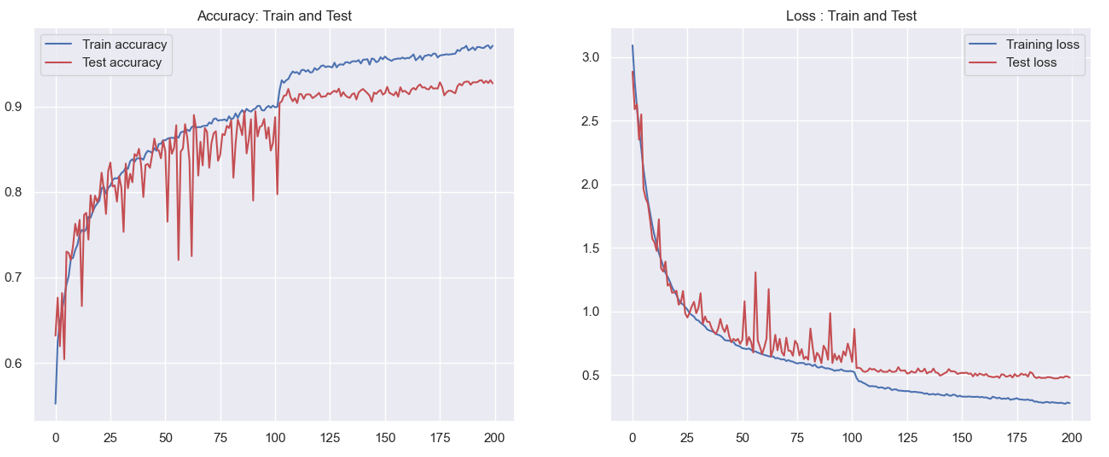
\includegraphics[width=0.45\linewidth]{model_cls_1.png}
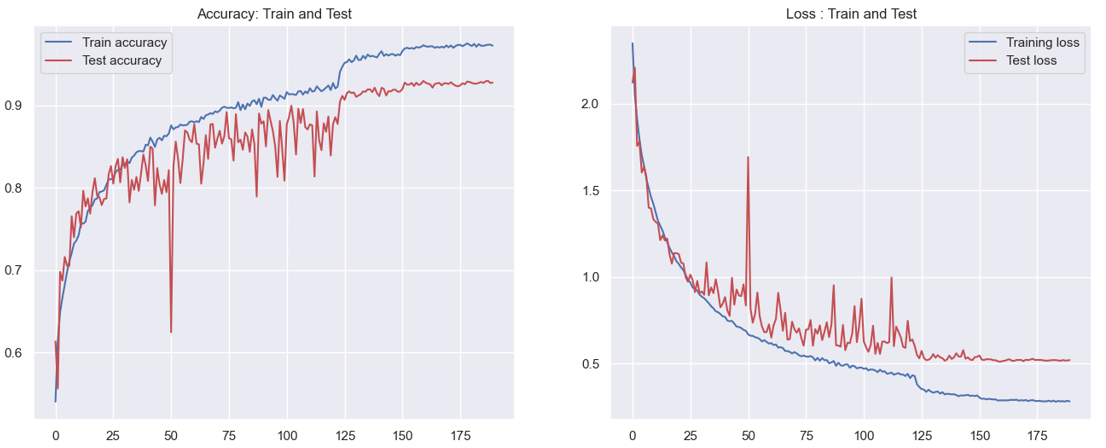
\includegraphics[width=0.45\linewidth]{model_cls_2.png}
\end{center}
\begin{itemize}
    \item Convergence stable pour les deux modèles
    \item Pas de sur-apprentissage (régularisation efficace)
    \item Modèle 2 : Arrêt précoce à 190 époques
\end{itemize}
\end{block}
}

\only<3>{
\begin{block}{Performances par Classe}
\begin{center}
\begin{tabular}{lcccccc}
\toprule
\multirow{2}{*}{\textbf{Classe}} & 
\multicolumn{3}{c}{\textbf{Modèle 1}} & 
\multicolumn{3}{c}{\textbf{Modèle 2}} \\ 
\cmidrule(lr){2-4} \cmidrule(lr){5-7}
& P & R & F1 & P & R & F1 \\
\midrule
Canette & 88.7 & 90.3 & 89.5 & 91.2 & 91.2 & 91.2 \\
Organique & 94.8 & 94.8 & 94.8 & 93.3 & 95.9 & 94.6 \\
Plastique & 89.1 & 87.9 & 88.5 & 91.0 & 87.7 & 89.3 \\
Textile & 96.6 & 97.1 & 96.9 & 94.5 & 96.8 & 95.6 \\
Verre & 94.1 & 93.7 & 93.9 & 93.8 & 92.5 & 93.1 \\
\bottomrule
\end{tabular}
\end{center}
\end{block}
}

\only<4>{
\begin{block}{Matrices de Confusion}
\begin{center}
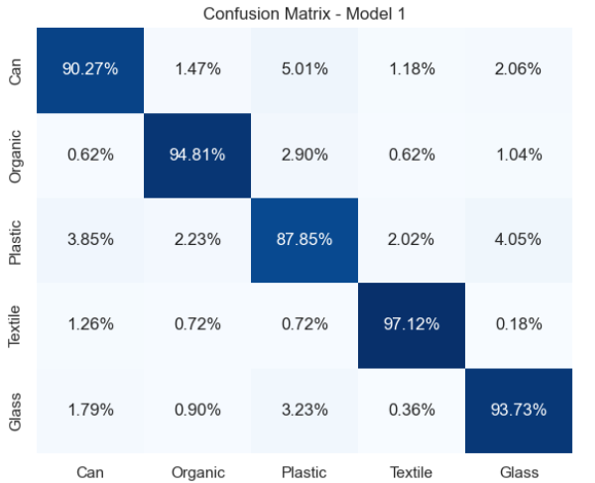
\includegraphics[width=0.45\linewidth]{matrix_1.png}
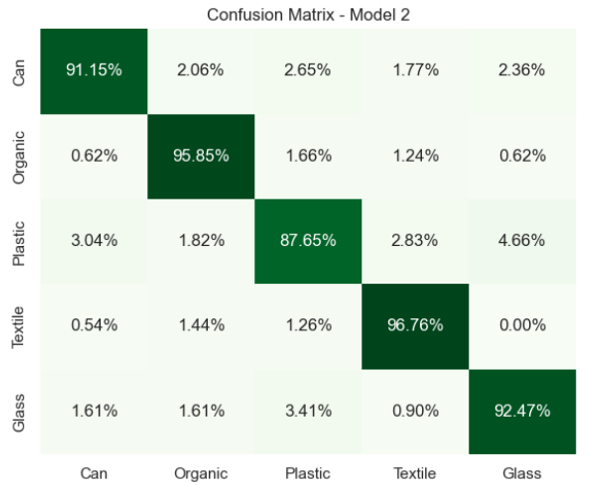
\includegraphics[width=0.45\linewidth]{matrix_2.png}
\end{center}
\begin{itemize}
    \item Forte diagonale pour les deux modèles
    \item Confusions mineures Canette/Plastique
    \item Excellente détection Textile/Organique
\end{itemize}
\end{block}
}

\only<5>{
\begin{block}{Synthèse des Performances}
\begin{center}
\begin{tabular}{lcc}
\toprule
\textbf{Métrique} & \textbf{Modèle 1} & \textbf{Modèle 2} \\
\midrule
Accuracy & 93.04\% & 92.96\% \\
Macro F1-score & 92.70\% & 92.76\% \\
Paramètres & 3,806,525 & 562,493 \\
Ratio légèreté & 1× & 6.8× \\
\bottomrule
\end{tabular}
\end{center}
\end{block}

\begin{alertblock}{Conclusion}
\begin{itemize}
    \item Performances très similaires (92\%)
    \item Modèle 2 : 7× plus léger avec performances équivalentes
    \item Choix optimal : Modèle 2 pour déploiement réel
\end{itemize}
\end{alertblock}
}

\end{frame}
\begin{frame}{Évaluation sur Données Locales}

\only<1>{
\begin{block}{Problème de Généralisation}
\begin{itemize}
    \item Performance initiale décevante : F1 < 68\% (sauf canette ~80\%)
    \item Écart entre données d'entraînement (idéalisées) et réalité terrain
    \item Images locales : résolution variable, objets multiples, cadrages complexes
\end{itemize}
\end{block}

\begin{alertblock}{Limites des Bases Publiques}
\begin{itemize}
    \item Images bien centrées, haute résolution
    \item Objet unique par image
    \item Conditions non représentatives du contexte réel
\end{itemize}
\end{alertblock}
}

\only<2>{
\begin{block}{Solution : Transfert Learning}
\begin{itemize}
    \item Réutilisation du modèle initial comme point de départ
    \item Entraînement des 3 dernières couches seulement
    \item 200 images/classe + 70\% données locales pour l'affinage
    \item 30\% données locales réservées pour l'évaluation finale
\end{itemize}
\end{block}

\begin{center}
\begin{tabular}{lc}
\toprule
\textbf{Élément} & \textbf{Description} \\
\midrule
Données d'affinage & 70\% données locales \\
Données de test & 30\% données locales \\
Renfort & 20 images/classe des tests initiaux \\
Prétraitement & Identique à l'entraînement initial \\
\bottomrule
\end{tabular}
\end{center}
}

\only<3>{
\begin{block}{Courbes d'Apprentissage après Transfert}
\begin{center}
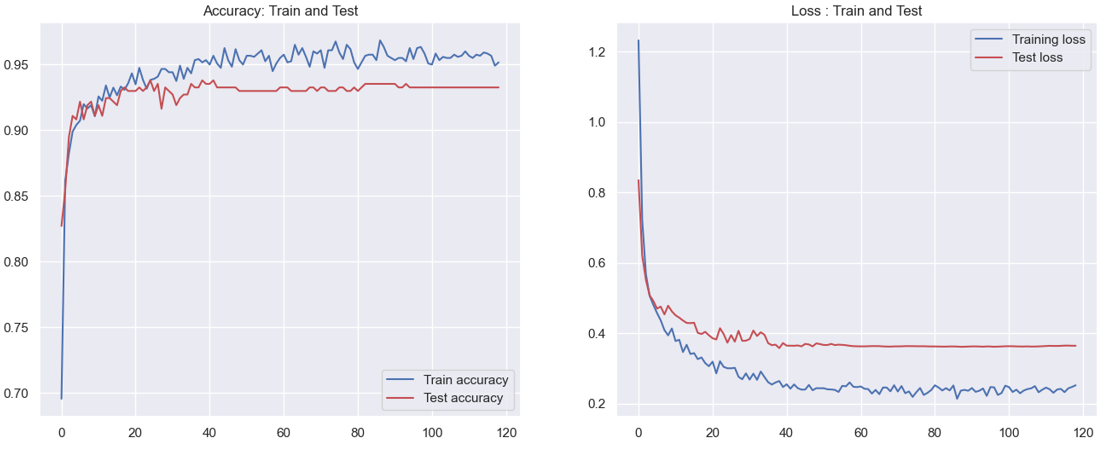
\includegraphics[width=0.45\linewidth]{plot_cls_n_13.png}
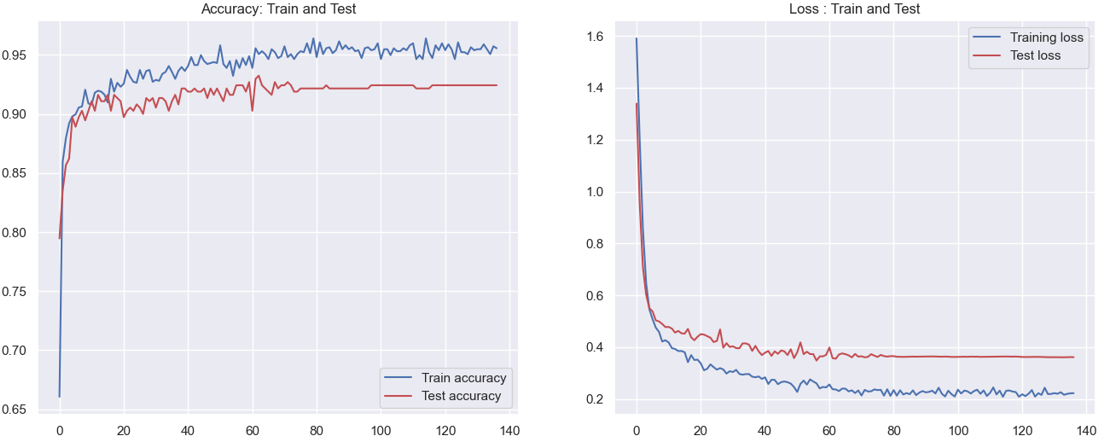
\includegraphics[width=0.45\linewidth]{plot_cls_n_14.png}
\end{center}
\begin{itemize}
    \item Convergence rapide grâce au transfert learning
    \item Adaptation efficace aux spécificités locales
    \item Stabilité de l'apprentissage
\end{itemize}
\end{block}
}

\only<4>{
\begin{block}{Résultats après Transfert Learning}
\begin{center}
\begin{tabular}{lccc}
\toprule
\textbf{Classe} & \textbf{Modèle 1 F1} & \textbf{Modèle 2 F1} \\
\midrule
Canette & 91.6\% & 93.8\% \\
Organique & 88.6\% & 89.2\% \\
Plastique & 85.7\% & 81.8\% \\
Textile & 74.1\% & 70.4\% \\
Verre & 90.5\% & 88.4\% \\
\midrule
Accuracy & 86.5\% & 85.3\% \\
Macro F1 & 86.1\% & 84.7\% \\
\bottomrule
\end{tabular}
\end{center}
\end{block}
}

\only<5>{
\begin{block}{Matrices de Confusion - Données Locales}
\begin{center}
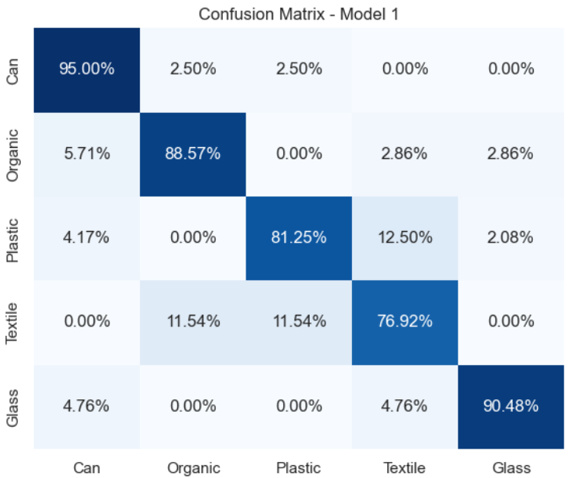
\includegraphics[width=0.45\linewidth]{matrix_n_1.png}
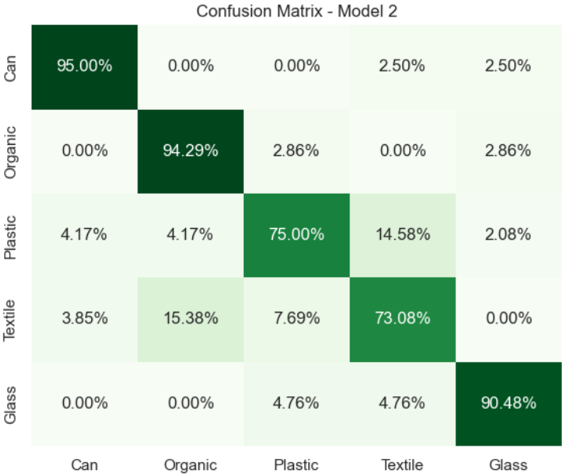
\includegraphics[width=0.45\linewidth]{matrix_n_2.png}
\end{center}
\begin{itemize}
    \item Amélioration significative après transfert learning
    \item Réduction des erreurs de classification
    \item Meilleure adaptation au contexte local
\end{itemize}
\end{block}
}

\only<6>{
\begin{block}{Comparaison Avant/Après Transfert}
\begin{center}
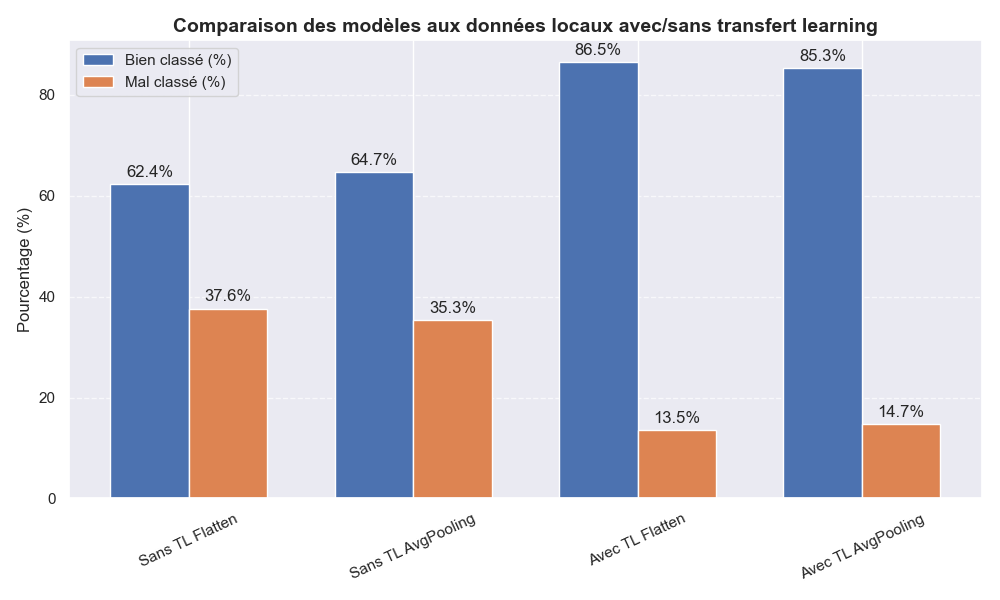
\includegraphics[width=0.6\linewidth]{comp.png}
\end{center}
\begin{itemize}
    \item Gain important en précision de classification
    \item Réduction du taux d'erreur
    \item Validation de l'approche par transfert learning
\end{itemize}
\end{block}
}

\end{frame}
\section{Approche avec le modèle JEPA}
\begin{frame}{Approche avec le modèle JEPA}
	\centering
	\vspace{0.5cm}
	
	\only<1>{
		\Huge
		\textcolor{mlblue}{\faIcon{project-diagram}}
		\vspace{0.5cm}
		
		\textbf{APPROCHE AVEC LE MODÈLE JEPA}
		\vspace{0.3cm}
		
		\normalsize
		Joint Embedding Predictive Architecture
	}
	
\end{frame}
\section{Améliorations du Système}
\begin{frame}{Améliorations du Système}
    \centering
    \vspace{0.5cm}
    
    % Titre principal
    \only<1>{
        \Huge
        \textcolor{mlblue}{\faIcon{rocket}}
        \vspace{0.5cm}
        
        \textbf{AMÉLIORATIONS DU SYSTÈME}
        \vspace{0.3cm}
        
        \normalsize
        Optimisation et perfectionnement de la solution
    }
\end{frame}
\subsection{Amélioration de la Classification}
\begin{frame}{Amélioration de la Classification}

\only<1>{
\begin{block}{Constat et Défis}
\begin{itemize}
    \item Essor des méthodes de classification pour le tri automatisé
    \item Résultats satisfaisants mais limites en contexte réel
    \item Problèmes de généralisation sur données variées
    \item Erreurs face à des situations complexes ou nouvelles
\end{itemize}
\end{block}

\begin{alertblock}{Objectif}
\begin{itemize}
    \item Analyser les limitations identifiées
    \item Proposer des stratégies d'amélioration
    \item Renforcer précision et adaptabilité en conditions réelles
\end{itemize}
\end{alertblock}
}

\only<2>{
\begin{block}{Facteurs Limitants}
\begin{itemize}
    \item \textbf{Faible volume} de données locales disponibles
    \item \textbf{Déséquilibre persistant} avec données publiques
    \item Modèle influencé par les caractéristiques dominantes
\end{itemize}
\end{block}

\begin{block}{Stratégie d'Amélioration}
\begin{itemize}
    \item \textbf{Équilibre optimal} entre données locales et publiques
    \item Données locales : adaptation au contexte réel
    \item Données publiques : diversité et stabilité
    \item Recherche de complémentarité pour une robustesse durable
\end{itemize}
\end{block}
}
\end{frame}
\subsection{Détection d'Anomalies}
\begin{frame}{Détection d'Anomalies}

\only<1>{
\begin{block}{Problème Identifié}
\begin{itemize}
    \item Modèles de classification limités aux classes connues
    \item Fausses prédictions inévitables pour déchets inconnus
    \item Impact critique sur les projets de valorisation (biogaz, électricité)
    \item Risque environnemental et économique
\end{itemize}
\end{block}

\begin{block}{Solution Proposée}
Intégration de mécanismes de détection d'anomalies avant classification
\end{block}
}

\only<2>{
\begin{block}{Deux Approches Explorées}
\begin{itemize}
    \item \textbf{Autoencodeur} : Détection basée sur l'erreur de reconstruction
    %\item \textbf{Discriminateur GAN} : Distinction données connues/inconnues
\end{itemize}
\end{block}

\begin{block}{Base de Données d'Évaluation}
\begin{itemize}
    \item 4 000 images de test (2 000 connues + 2 000 inconnues)
    \item Données inconnues : batteries, cartons, autres déchets
    \item Simulation de contexte réaliste avec nouvelles catégories
\end{itemize}
\end{block}
}

\end{frame}

\begin{frame}{Détection par Autoencodeur Variationnel ($\beta$-VAE)}

\only<1>{
\begin{block}{Principe et Architecture}
\begin{itemize}
    \item Autoencodeur entraîné sur données "normales"
    \item Détection par erreur de reconstruction
    \item Architecture $\beta$-VAE résiduelle ($\beta = 0.001$)
    \item Espace latent: 128 dimensions
\end{itemize}
\end{block}

\begin{center}
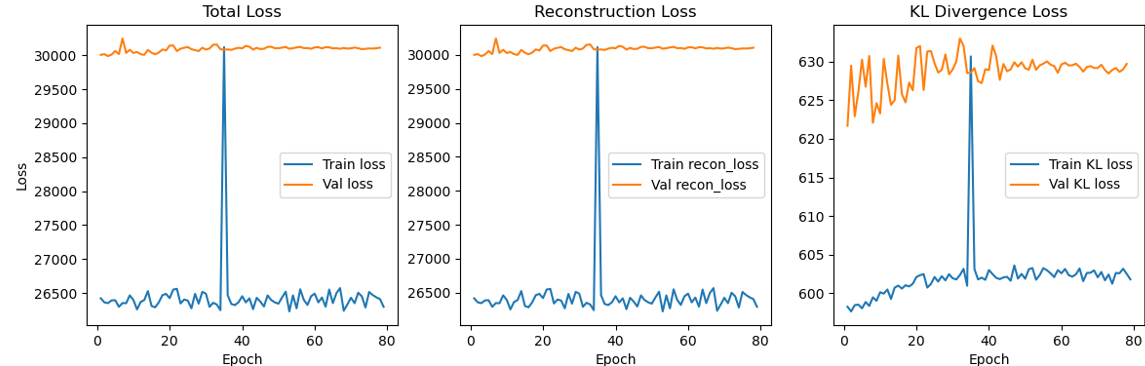
\includegraphics[width=0.8\linewidth]{autoencoder.png}
\end{center}
\begin{center}
\small Courbe d'apprentissage montrant le surapprentissage
\end{center}
} % Fin du only<1>

\only<2>{
\begin{block}{Exemples de Reconstruction}
\begin{center}
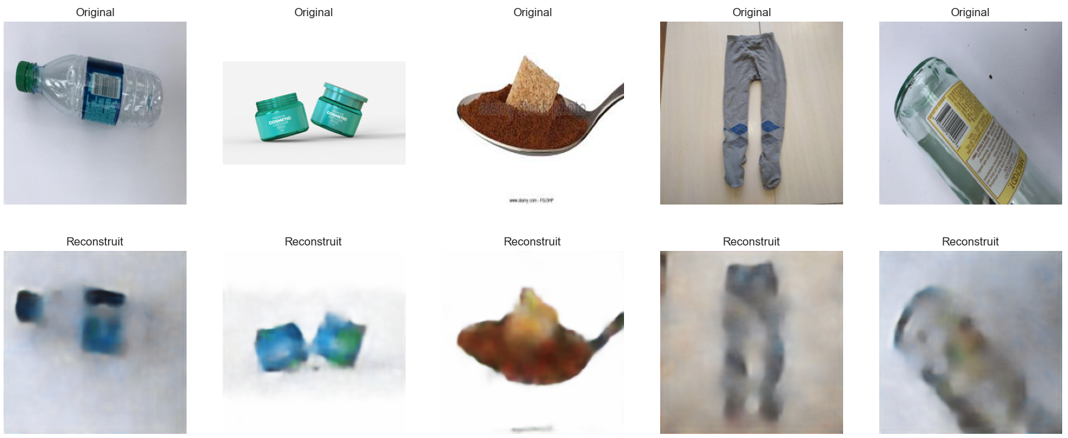
\includegraphics[width=0.5\linewidth]{train_auto.png}
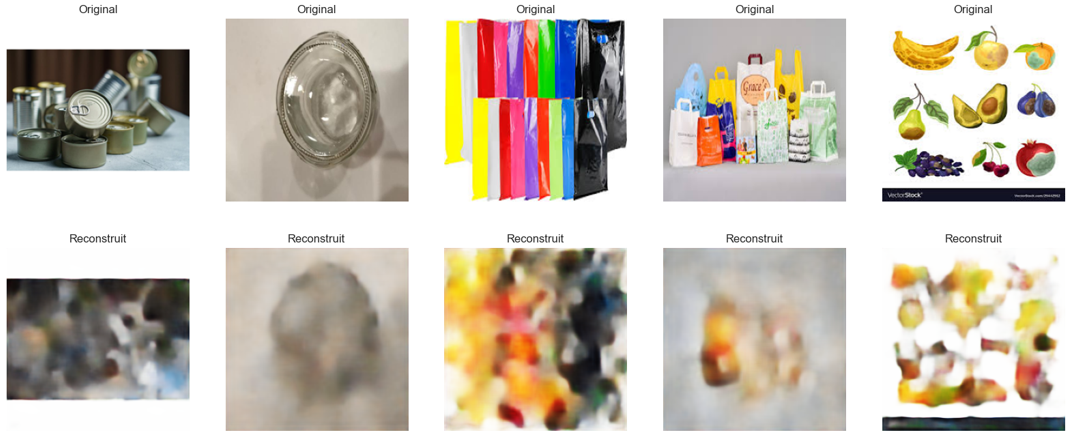
\includegraphics[width=0.5\linewidth]{test_auto.png}
\end{center}
\begin{center}
\small Haut: entraînement - Bas: test (reconstructions imprécises)
\end{center}
\end{block}
} % Fin du only<2>

\only<3>{
\begin{block}{Optimisation du Seuil}
\begin{center}
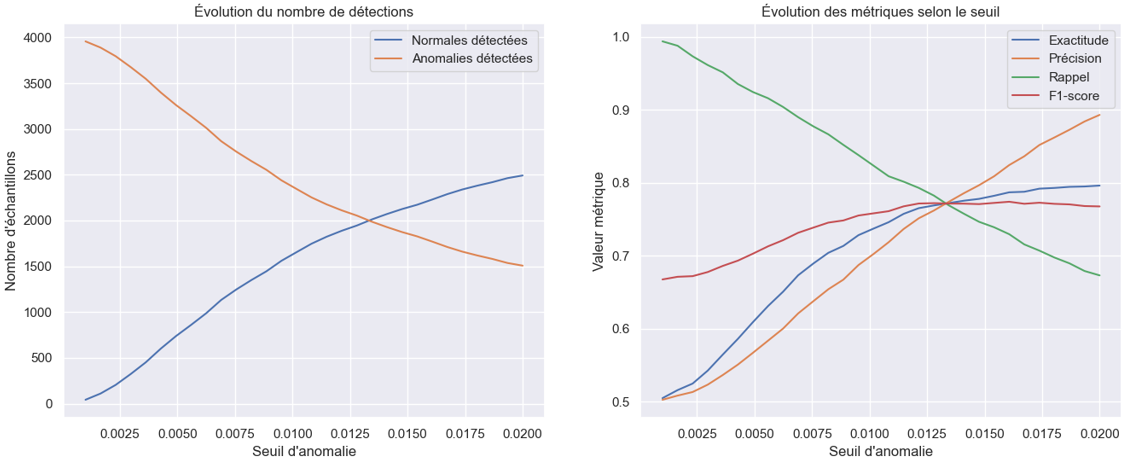
\includegraphics[width=0.9\linewidth]{auto_metric.png}
\end{center}
\begin{center}
\small Évolution des métriques en fonction du seuil (optimal: 0.01607)
\end{center}
\end{block}
} % Fin du only<3>
\only<4>{
\begin{block}{Résultats et Performance}
\begin{center}
\begin{tabular}{lccc}
\hline
\textbf{Classe} & \textbf{Précision} & \textbf{Rappel} & \textbf{F1-score} \\
\hline
Normal & 75.7\% & 84.4\% & 79.8\% \\
Anormal & 82.4\% & 73.0\% & 77.4\% \\
\hline
\end{tabular}
\end{center}
\end{block}
\begin{center}
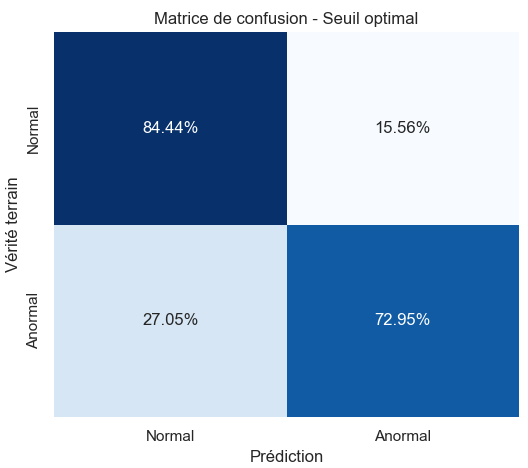
\includegraphics[width=0.5\linewidth]{matrix_auto.png}
\end{center}
\begin{center}
\small Matrice de confusion - Performance correcte mais perfectible
\end{center}
} % Fin du only<4>

\end{frame}

\section{Conclusion}
\begin{frame}{\faIcon{compass} Conclusion}

    \centering
    \vspace{1cm}
    
    \only<1>{
        \Huge
        \textcolor{mlblue}{\faIcon{compass}}
        \vspace{0.5cm}
        
        \textbf{CONCLUSION}
        \vspace{1cm}
        
        \Large
        Pour donner des éléments de conclusion,
        \vspace{0.3cm}
        
        \normalsize
        ce travail montre une belle opportunité d'automatiser \\
        le tri des déchets avec des modèles de Deep Learning
    }
   
    \only<2>{
        \vspace{1.5cm}
        
        \LARGE
        \textcolor{orange}{\faIcon{road}}
        \vspace{0.5cm}
        
        \textbf{Mais pour y arriver...}
        \vspace{0.8cm}
        
        \Large
        \textcolor{gray}{il nous reste encore un bout de chemin à parcourir}
        \vspace{0.5cm}
        
        \begin{tikzpicture}
            \draw[gray, thick] (0,0) -- (8,0);
            \draw[mlblue, thick] (0,0) -- (3,0);
            \fill[mlblue] (3,0) circle (0.1);
        \end{tikzpicture}
        
        \vspace{0.3cm}
        \small
        \textcolor{mlblue}{Progrès accomplis} \hfill \textcolor{gray}{Chemin restant}
    }
\end{frame}
\section*{Remerciements}
\begin{frame}{Remerciements}
    
    \only<1>{
        \centering
        \vspace{1.5cm}
        
        \Huge
       
        \textbf{Je vous remercie du fond du cœur} \\
        \vspace{0.3cm}
        \Large
        pour votre attention et votre présence
    }
    
   
\end{frame}
\end{document}